\documentclass[solution,addpoints,12pt]{exam}
\usepackage{amsmath}
\usepackage{mathtools}
\usepackage{amsthm}
\usepackage{amssymb}
\usepackage{tikz}
\usepackage{animate}
\usepackage{hyperref}
\usepackage{booktabs}
\newtheorem{theorem}{Theorem}
\newtheorem{lemma}[theorem]{Lemma}
\DeclarePairedDelimiter\ceil{\lceil}{\rceil}

\newenvironment{Solution}{\begin{EnvFullwidth}\begin{solution}}{\end{solution}\end{EnvFullwidth}}

\printanswers
%\unframedsolutions
\pagestyle{headandfoot}

%%%%%%%%%%%%%%%%%%%%%%%%%%%%%%%%%%%%%%%%%%%%%%%%%%%%%%
%%%%%%%%%%%%%%%%%%% INSTRUCTIONS %%%%%%%%%%%%%%%%%%%%%
% * Fill in your name and roll number below

% * Answer in place (after each question)

% * Use \begin{solution} and \end{solution} to typeset
%   your answers.
%%%%%%%%%%%%%%%%%%%%%%%%%%%%%%%%%%%%%%%%%%%%%%%%%%%%%%
%%%%%%%%%%%%%%%%%%%%%%%%%%%%%%%%%%%%%%%%%%%%%%%%%%%%%%

% Fill in the details below
\def\studentName{\textbf{Name: Anant Shah\hspace{1mm}}}
\def\studentRoll{\textbf{Roll No: EE16B105\hspace{1mm}}}

\firstpageheader{CS 7015 - Deep Learning - Assignment 1}{}{\studentName, \studentRoll}
\firstpageheadrule

\newcommand{\brac}[1]{\left[ #1 \right]}
\newcommand{\curly}[1]{\left\{ #1 \right\}}
\newcommand{\paren}[1]{\left( #1 \right)}
\newcommand{\card}[1]{\left\lvert #1 \right\rvert}

\begin{document}
\textbf{Instructions:}
\begin{itemize}
    \itemsep0em
    \item This assignment is meant to help you grok certain concepts we will use in the course. Please don't copy solutions from any sources.
    \item Avoid verbosity.
    \item The assignment needs to be written in latex using the attached tex file. The solution for each question should be written in the solution block in space already provided in the tex file. \textbf{Handwritten assignments will not be accepted.}
    
\end{itemize}

\begin{questions}

\question \textbf{Partial Derivatives}
          \newline
          \begin{parts}
   

        \part Find the derivative of $g(\rho)$ with respect to $\rho$ where $g(\rho)$ is given by,
      \[ g(\rho) = \frac{1}{2} \rho log\frac{\rho}{\rho+\hat{\rho}} + \frac{1}{2} \hat{\rho} log\frac{\hat{\rho}}{\rho+\hat{\rho}} \]
      (You can consider $\hat{\rho}$ as constant)
      \begin{solution}
      %\vspace*{50mm}
      \[\frac{\partial g(\rho)}{\partial \rho} = \frac{1}{2} \frac{\partial \rho log\frac{\rho}{\rho+\hat{\rho}}}{\partial \rho} + \frac{1}{2} \frac{\partial \hat{\rho} log\frac{\hat{\rho}}{\rho+\hat{\rho}}}{\partial \rho}\]
      \[\implies \frac{\partial g(\rho)}{\partial \rho} = \frac{1}{2} log\frac{\rho}{\rho+\hat{\rho}} + \frac{1}{2} \rho (\frac{1}{\rho}-\frac{1}{\rho+\hat{\rho}}) - \frac{1}{2} \frac{\hat{\rho}}{\rho+\hat{\rho}}\]
      \[\implies \frac{\partial g(\rho)}{\partial \rho} = \frac{1}{2} log\frac{\rho}{\rho+\hat{\rho}} + \frac{1}{2} \frac{\hat{\rho}}{\rho+\hat{\rho}} - \frac{1}{2} \frac{\hat{\rho}}{\rho+\hat{\rho}} \]
      \[\implies \frac{\partial g(\rho)}{\partial \rho} = \frac{1}{2} log\frac{\rho}{\rho+\hat{\rho}} \]
      \end{solution}
            \part Consider the following computation ,
                  \begin{center}
                  \hspace*{-15mm}
                    \tikzstyle{neuron1}=[circle,draw=blue!50,fill=blue!20,thick,minimum size=1mm]
                    \tikzstyle{neuron2}=[circle,draw=blue!50,fill=blue!20,thick,minimum size=6mm]
                    \tikzstyle{input}=[circle,draw=black!50,fill=black!20,thick,minimum size=6mm]
                    \begin{tikzpicture}
                        \node [neuron1] (neuron1) at (0.1,6)  {$\frac{1 + tanh(wx+b)}{2}$} ;
                        \node [neuron2] (neuron2) at (4,6)  {$sigm(z)$} ;
                        \node (input1) at (-3,6)  {$x$};
                        \node (input0) at (-3,5)  {$1$};
                        \node (output0) at (6,6)  {$f(x)$};
                        \node (formula) at (0,4) {where $ z = \frac{1 + tanh(wx+b)}{2}$ and $f(x) = sigm(z)$};
                        \node (formula2) at (0,3) {by definition : $sigm(z) = \frac{1}{1+e^{-z}}$ and $tanh(z) = \frac{e^{z} - e^{-z}}{e^{z} + e^{-z}} $ };
                        \draw [->] (input0) -- (neuron1);
                        \draw [->] (input1) -- (neuron1);
                        \draw[->] (neuron1) -- (neuron2);
                        \draw [->] (neuron2) -- (output0);
                        \node (label) at (2.3,6.3) {$z$};
                    \end{tikzpicture}
                  \end{center}
                  The value $L$ is given by, 
                  \[ 
                     L = - y \log (f(x))          \]
                  Here, $x$ and $y$ are constants and $w$ and $b$ are parameters that can be modified.
                  In other words, $L$ is a function of $w$ and $b$.

                  Derive the partial derivatives, $\frac{\partial L}{\partial w}$ and $\frac{\partial L}{\partial b}$.
   
              \begin{solution}
              \[\frac{\partial L}{\partial w} = -\frac{y}{f(x)} \frac{\partial f(x)}{\partial w}\]
              \[\implies \frac{\partial L}{\partial w} = -\frac{y}{f(x)} \frac{\partial f(x)}{\partial z} \frac{\partial z}{\partial w}\]
              \[z = \frac{1+\frac{e^{wx+b}-e^{-(wx+b)}}{e^{wx+b}+e^{-(wx+b)}}}{2}\]
              \[\implies z = \frac{1}{1+e^{-2(wx+b)}}\]
              \[\frac{\partial L}{\partial w} = -\frac{y}{f(x)} \frac{e^{-z}}{(1+e^{-z})^2} \frac{\partial \frac{1}{1+e^{-2(wx+b)}}}{\partial w}\]
              \[\implies \frac{\partial L}{\partial w} = -\frac{ye^{-z}}{(1+e^{-z})} \frac{2x}{(e^{wx+b}+e^{-(wx+b)})^2}\]
              \[\frac{\partial L}{\partial b} = -\frac{y}{f(x)} \frac{\partial f(x)}{\partial b}\]
              \[\implies \frac{\partial L}{\partial b} = -\frac{y}{f(x)} \frac{\partial f(x)}{\partial z} \frac{\partial z}{\partial b}\]
              \[\implies \frac{\partial L}{\partial b} = -\frac{y}{f(x)} \frac{e^{-z}}{(1+e^{-z})^2} \frac{\partial \frac{1}{1+e^{-2(wx+b)}}}{\partial b}\]
              \[\implies \frac{\partial L}{\partial b} = -\frac{ye^{-z}}{(1+e^{-z})} \frac{2}{(e^{wx+b}+e^{-(wx+b)})^2}\]
              \end{solution}

         \end{parts}  
         

\question 
\textbf{Chain Rule}:
    \begin{parts}
            \part Consider the evaluation of $E$ as given below,
                  \[
                    E = h(u,v,w,x) = 2*f(au + bv) - g(cw + dx))
                  \]
                  \begin{minipage}{0.45\linewidth}
                  Represented as graph:\\
                  \includegraphics[scale=0.5]{download.png}
                  \end{minipage}\quad
                  \begin{minipage}{0.55\linewidth}
                  Here $u,v,w,x$ are inputs (constants) and $a,b,c,d$ are parameters (variables). $f$ and $g$ are the activation functions (with $z$ as input) defined as below:
                  \begin{eqnarray*}
                  f(z) = sigm(z) \qquad \qquad g(z) = tanh(z)
                  \end{eqnarray*}
                  \end{minipage}\\                  
                  Note that here $E$ is a function of parameters $a,b,c,d$.
                  Compute the partial derivatives of $E$ with respect to the parameters $a$, $b$, $c$ and $d$ \textit{i.e.} $\frac{\partial E}{\partial a}$, $\frac{\partial E}{\partial b}$, $\frac{\partial E}{\partial c}$ and $\frac{\partial E}{\partial d}$.
                  \begin{solution}
                  \[f(au+bv) = \frac{1}{1+e^{-(au+bv)}}\]
                  \[g(cw+dx) = \frac{e^{cw+dx}-e^{-(cw+dx)}}{e^{cw+dx}+e^{-(cw+dx)}}\]
                  \[\frac{\partial E}{\partial a} = 2\frac{\partial f(au+bv)}{\partial a} - \frac{\partial g(cw+dx)}{\partial a}\]
                  \[\implies \frac{\partial E}{\partial a} = 2\frac{\partial f(au+bv)}{\partial (au+bv)} \frac{\partial (au+bv)}{\partial a} + 0\]
                  \[\implies \frac{\partial E}{\partial a} = 2\frac{e^{-(au+bv)}}{(1+e^{-(au+bv)})^2} u\]
                  \[\frac{\partial E}{\partial b} = 2\frac{\partial f(au+bv)}{\partial b} - \frac{\partial g(cw+dx)}{\partial b}\]
                  \[\implies \frac{\partial E}{\partial b} = 2\frac{\partial f(au+bv)}{\partial (au+bv)} \frac{\partial (au+bv)}{\partial b} + 0\]
                  \[\implies \frac{\partial E}{\partial b} = 2\frac{e^{-(au+bv)}}{(1+e^{-(au+bv)})^2} v\]
                  \[\frac{\partial E}{\partial c} = 2\frac{\partial f(au+bv)}{\partial c} - \frac{\partial g(cw+dx)}{\partial c}\]
                  \[\implies \frac{\partial E}{\partial c} = 0 - \frac{\partial g(cw+dx)}{\partial (cw+dx)} \frac{\partial(cw+dx)}{\partial c}\]
                  \[\implies \frac{\partial E}{\partial c} = - \frac{(e^{cw+dx}+e^{-(cw+dx)})^2-(e^{cw+dx}-e^{-(cw+dx)})^2}{(e^{cw+dx}+e^{-(cw+dx)})^2} w\]
                  \[\implies \frac{\partial E}{\partial c} = \frac{-4w}{(e^{cw+dx}+e^{-(cw+dx)})^2}\]
                  \[\frac{\partial E}{\partial d} = 2\frac{\partial f(au+bv)}{\partial d} - \frac{\partial g(cw+dx)}{\partial d}\]
                  \[\implies \frac{\partial E}{\partial d} = 0 - \frac{\partial g(cw+dx)}{\partial (cw+dx)} \frac{\partial(cw+dx)}{\partial d}\]
                  \[\implies \frac{\partial E}{\partial d} = - \frac{(e^{cw+dx}+e^{-(cw+dx)})^2-(e^{cw+dx}-e^{-(cw+dx)})^2}{(e^{cw+dx}+e^{-(cw+dx)})^2} x\]
                  \[\implies \frac{\partial E}{\partial d} = \frac{-4x}{(e^{cw+dx}+e^{-(cw+dx)})^2}\]
                  \end{solution}
            \part Assume that $z = f(x, y)$, where $x = uv$ and $y = \frac{u}{v}$. We use $f_{x}$ to denote the partial derivative $\frac{\partial f}{\partial x}$. Using the chain rule, express  $\frac{\partial z }{\partial u}$ and  $\frac{\partial z }{\partial v}$ in terms of $u$, $v$, $f_{x}$ and $f_{y}$. 
        \begin{solution}
        \[\frac{\partial z}{\partial u} = \frac{\partial z}{\partial x}\frac{\partial x}{\partial u} + \frac{\partial z}{\partial y}\frac{\partial y}{\partial u}\]
        \[\implies \frac{\partial z}{\partial u} = f_{x}v + \frac{f_y}{v}\]
        \[\frac{\partial z}{\partial v} = \frac{\partial z}{\partial x}\frac{\partial x}{\partial v} + \frac{\partial z}{\partial y}\frac{\partial y}{\partial v}\]
        \[\implies \frac{\partial z}{\partial u} = f_{x}u - \frac{uf_y}{v^2}\]
        \end{solution}
            
    
    \part Given the change of variables as mentioned in the previous part: $x = uv$ and $y = \frac{u}{v}$, calculate the Jacobian of this transformation.
    \begin{solution}
    The Jacobian matrix $J$ is given by :
    \[ J =
    \begin{bmatrix}
    \frac{\partial x}{\partial u} & \frac{\partial x}{\partial v} \\
    \frac{\partial y}{\partial u} & \frac{\partial y}{\partial v}
    \end{bmatrix}
    \]
    \[\implies J =
    \begin{bmatrix}
    v & u \\
    \frac{1}{v} & \frac{-u}{v^2}
    \end{bmatrix}
    \]
    The Jacobian determinant is given by $det(J)$ where $J$ is the Jacobian matrix
    \[det(J) = \frac{-u}{v}-\frac{u}{v}\]
    \[det(J)\ = -2\frac{u}{v}\]
    \end{solution}
    \part Calculate the Jacobian of the transformation for rectangular coordinates; \textit{i.e.}, the Jacobian of $x$ = $r sin \theta$, $y$ = $r cos \theta$, $z$ = $z$, (hint: using the relevant partial derivatives)
    \begin{solution}
    The Jacobian matrix $J$, is given by :
    \[ J =
    \begin{bmatrix}
    \frac{\partial x}{\partial r} & \frac{\partial x}{\partial \theta} & \frac{\partial x}{\partial z} \\
    \frac{\partial y}{\partial r} & \frac{\partial y}{\partial \theta} & \frac{\partial y}{\partial z} \\
    \frac{\partial z}{\partial r} & \frac{\partial z}{\partial \theta} & \frac{\partial z}{\partial z} \\
    \end{bmatrix}
    \]
    \[ J =
    \begin{bmatrix}
    sin(\theta) & rcos(\theta) & 0 \\
    cos(\theta) & -rsin(\theta) & 0 \\
    0 & 0 & 1 \\
    \end{bmatrix}
    \]
    The Jacobian determinant is given by $det(J)$ where $J$ is the Jacobian matrix 
    \[det(J) = -rsin^2(\theta) -rcos^2(\theta)\]
    \[det(J) = -r\]
    \end{solution}
    \end{parts}
\question  \textbf{Visit Taylor Series} The first order derivative of a function $f$ is defined by the following limit,
          \begin{equation} \label{eq:deriv_definition}
            \frac{df(x)}{dx} = \lim_{h \to 0} \frac{f(x + h) - f(x)}{h}
          \end{equation}
          On observing the above definition we see that the derivative of a function is the ratio of
          change in the function value to the change in the function input, 
          when we change the input by a small quantity (infinitesimally small).
          A first degree approximation based on eq. \ref{eq:deriv_definition} would be the following.
          \begin{equation}
            f(x+h) \approx f(x) + h \frac{df(x)}{dx}
          \end{equation}
          Consider $f(x) = ln(x+5)$. 
         \begin{parts}
         \part
          Estimate the value of $f(1)$,$f(1.1)$ and $f(2.5)$ using the above formula.
                \begin{solution}
                Let us approximate the function around the point $x_{o} = e-5$
                \[f(1) = f(e-5+6-e) \approx f(e-5) + \frac{6-e}{e}\]
                \[f(1) \approx \frac{6}{e} = 2.207\]
                \[f(1.1) = f(e-5+6.1-e) \approx f(e-5) + \frac{6.1-e}{e}\]
                \[f(1.1) \approx \frac{6.1}{e} = 2.244\]
                \[f(2.5) = f(e-5+7.5-e) \approx f(e-5) + \frac{7.5-e}{e}\]
                \[f(2.5) \approx \frac{7.5}{e} = 2.759\]
                \end{solution}
          \part Compare these estimates to the actual values of function $f(1)$,$f(1.1)$ and $f(2.5)$. Explain the discrepancy as we increase the value.
                \begin{solution}
                Let the approximation above be f'(x).\newline
                \[f'(1) - f(1) = 2.207 - 1.792 = 0.415\]
                \[f'(1.1) - f(1) = 2.244 - 1.808 = 0.436\]
                \[f'(2.5) - f(2.5) = 2.759 - 2.015 = 0.744\]
                We can clearly see that the error is increasing as we increase the value of $h$. What we are essentially doing with the above approximation is linearizing the function about a point $x_{o}$. However, the log function is not linear. This is a first order approximation and hence there is a mismatch in the values. As we move away from $x_{o}$, the $h$ value is increasing. But the first order approximation is only valid for infinitesimal $h$, hence a discrepancy in the value.
                \end{solution}
          \part Can we get a better estimate of $f(1)$,$f(1.1)$ and $f(2.5)$ ? How?
                \begin{solution}
                Yes,we can get a better approximation by using higher order terms in the Taylor series equation
                \[f(x_{o}+h) = f(x_{o}) + h\frac{df(x_{o})}{dx} + \frac{h^2}{2!}\frac{d^2f(x_{o})}{dx^2} + \dots\]
                Or if we still want to use the first order approximation, then we need to choose a point which is infinitesimally close to the function argument and approximate it around that point.
                \end{solution}
            
        \part Consider $g(x) = a + be^{x} + c*\cos(x)$. Find a, b, c $\in$ R such that $g$ approximates $f$ at
$x$ = 0. (i.e. by matching the (i) direct values (ii) first derivative and (iii) second derivative at $x = 0$).
        \begin{solution}
        \[g(x) = a + be^{x} + ccos(x)\]
        Using Taylor Series approximation, we can approximate the functions around $x=0$ as
        \[g(x) \approx a + b(1 + \frac{x}{1!} + \frac{x^2}{2!} + \dots) + c(1-\frac{x^2}{2!} + \frac{x^4}{4!} + \dots)\]
        An approximation for $f$ around x=0 using Taylor Series is
        \[f(x) \approx ln(5) + \frac{x}{5} - \frac{x^2}{25.2!} + \dots\]
        Mathcing the respective derivative values, we obtain the following equations
        \[a + b + c = ln(5)\]
        \[b = \frac{1}{5} = 0.2\]
        \[\frac{b-c}{2} = \frac{-1}{50}\]
        \[\implies c = \frac{6}{25} = 0.24\]
        \[\implies a = ln(5) - \frac{11}{25} = 1.169\]
        \end{solution}
          
\end{parts}

\question
\textbf{Differentiation of function of multiple variables}
          \begin{equation*}
            \begin{aligned}
              s_1 & = tan(w_1 x) \\
              s_2 & = sec(w_2 x + s_1) \\
              s_3 & = sin(w_3 s_1 + w_4 s_2) \\
              s_4 & = cos(w_5 s_3 + w_6) \\
              y   & = tanh(w_7 s_4 + w_8)
            \end{aligned}
          \end{equation*}

          An alternative representation of the function $y$ is given in the figure below.
          \begin{center}
            \includegraphics[scale=0.7]{fig2.png}
          \end{center}

          Compute the derivatives $\frac{dy}{dw_1}$ and $\frac{dy}{dw_2}$ (show all the steps).

          \begin{solution}
          \[\frac{dy}{dw_{1}} = \frac{\partial y}{\partial (w_{7}s_{4}+w_{8})} \frac{\partial (w_{7}s_{4}+w_{8})}{\partial w_{1}}\]
          \[\implies \frac{dy}{dw_{1}} = \frac{4}{(e^{w_{7}s_{4}+w_{8}}+e^{-(w_{7}s_{4}+w_{8})})^2} w_{7} \frac{\partial s_{4}}{w_{1}}\]
          \[\implies \frac{dy}{dw_{1}} = \frac{-4w_{7}w_{5}}{(e^{w_{7}s_{4}+w_{8}}+e^{-(w_{7}s_{4}+w_{8})})^2} sin(w_{5}s_{3}+w_{6}) \frac{\partial s_{3}}{\partial w_{1}}\]
          \[\implies \frac{dy}{dw_{1}} = \frac{-4sin(w_{5}s_{3}+w_{6})w_{7}w_{5}}{(e^{w_{7}s_{4}+w_{8}}+e^{-(w_{7}s_{4}+w_{8})})^2} cos(w_{3}s_{1}+w_{4}s_{2})(w_{3}\frac{\partial s_{1}}{\partial w_{1}}+w_{4}\frac{\partial s_{2}}{\partial w_{1}})\]
          
          \begin{multline*}
          \implies \frac{dy}{dw_{1}} = \frac{-4sin(w_{5}s_{3}+w_{6})cos(w_{3}s_{1}+w_{4}s_{2})w_{7}w_{5}}{(e^{w_{7}s_{4}+w_{8}}+e^{-(w_{7}s_{4}+w_{8})})^2} (w_{3}xsec^2(w_{1}x) + \\ w_{4}sec(w_{2}x+s_{1})tan(w_{2}x+s_{1})\frac{\partial (w_{2}x+s_{1})}{\partial w_{1}}) \end{multline*}
          
          \begin{multline*}
          \implies \frac{dy}{dw_{1}} = \frac{-4sin(w_{5}s_{3}+w_{6})cos(w_{3}s_{1}+w_{4}s_{2})w_{7}w_{5}}{(e^{w_{7}s_{4}+w_{8}}+e^{-(w_{7}s_{4}+w_{8})})^2} (w_{3}xsec^2(w_{1}x) + \\ w_{4}sec(w_{2}x+s_{1})tan(w_{2}x+s_{1})(xsec^2(w_{1}x))) \end{multline*}
          
          \begin{multline*}
          \implies \frac{dy}{dw_{1}} = \frac{-4w_{7}w_{5}xsin(w_{5}s_{3}+w_{6})cos(w_{3}s_{1}+w_{4}s_{2})sec^2(w_{1}x)}{(e^{w_{7}s_{4}+w_{8}}+e^{-(w_{7}s_{4}+w_{8})})^2} (w_{3} + \\ w_{4}tan(w_{2}x+s_{1})sec(w_{2}x+s_{1}))
          \end{multline*}
          
          \[\frac{dy}{dw_{2}} = \frac{\partial y}{\partial (w_{7}s_{4}+w_{8})} \frac{\partial (w_{7}s_{4}+w_{8})}{\partial w_{2}}\]
          \[\implies \frac{dy}{dw_{2}} = \frac{4}{(e^{w_{7}s_{4}+w_{8}}+e^{-(w_{7}s_{4}+w_{8})})^2} w_{7} \frac{\partial s_{4}}{w_{2}}\]
          \[\implies \frac{dy}{dw_{2}} = \frac{-4w_{7}w_{5}}{(e^{w_{7}s_{4}+w_{8}}+e^{-(w_{7}s_{4}+w_{8})})^2} sin(w_{5}s_{3}+w_{6}) \frac{\partial s_{3}}{\partial w_{2}}\]
          \[\implies \frac{dy}{dw_{2}} = \frac{-4sin(w_{5}s_{3}+w_{6})w_{7}w_{5}}{(e^{w_{7}s_{4}+w_{8}}+e^{-(w_{7}s_{4}+w_{8})})^2} cos(w_{3}s_{1}+w_{4}s_{2})(w_{3}\frac{\partial s_{1}}{\partial w_{2}}+w_{4}\frac{\partial s_{2}}{\partial w_{2}})\]
          
          \begin{multline*}
          \implies \frac{dy}{dw_{2}} = \frac{-4sin(w_{5}s_{3}+w_{6})cos(w_{3}s_{1}+w_{4}s_{2})w_{7}w_{5}}{(e^{w_{7}s_{4}+w_{8}}+e^{-(w_{7}s_{4}+w_{8})})^2} (0 + \\ (w_{4}x)sec(w_{2}x+s_{1})tan(w_{2}x+s_{1})) \end{multline*}
          
          \[\implies \frac{dy}{dw_{2}} = \frac{-4(w_{7}w_{5}w_{4}x)sin(w_{5}s_{3}+w_{6})cos(w_{3}s_{1}+w_{4}s_{2})sec(w_{2}x+s_{1})tan(w_{2}x+s_{1})}{(e^{w_{7}s_{4}+w_{8}}+e^{-(w_{7}s_{4}+w_{8})})^2}\]
          
          \end{solution}
          
\question \textbf{Differentiation of vectors/matrices}
          \newline
          Consider vectors $\boldsymbol{u,b} \in \mathbb{R}^d$, and matrix $\boldsymbol{A} \in \mathbb{R}^{n \times n}$.
          \newline
          The derivative of a scalar $f$ w.r.t. a vector $\boldsymbol{u}$ is a vector by itself, given by
          \[
            \nabla f = \left( \frac{\partial f}{\partial u_1}, \frac{\partial f}{\partial u_2}, \dots, 
                         \frac{\partial f}{\partial u_n} 
                       \right)
          \]
          \newline
         ( \textbf{Hint}:  The derivative of a scalar $f$ w.r.t. a matrix $\boldsymbol{X}$, is a matrix whose $(i,j)$ component is $\frac{\partial f}{\partial X_{ij}}$, where $X_{ij}$ is the $(i,j)$ component of the matrix $\boldsymbol{X}$.)
         \newline
         \begin{parts}
         \part Derive the expression for the derivative:  $ \nabla \textbf{\textit{u}}^{T}\textbf{\textit{Au}} + \textbf{\textit{b}}^{T}\textbf{\textit{u}}$.
         \begin{solution}
         Let $\textbf{\textit{u}}^{T} = \begin{bmatrix} u_{1} & u_{2} & \dots & u_{n} \end{bmatrix}$, $\textbf{\textit{b}}^{T} = \begin{bmatrix} b_{1} & b_{2} & \dots & b_{n} \end{bmatrix}$ and \newline $ \textbf{\textit{A}} =
         \begin{bmatrix}
         A_{11} & A_{12} & \dots & A_{1n} \\
         A_{21} & A_{22} & \dots & A_{2n} \\
         \vdots & \vdots & \ddots & \vdots \\
         A_{n1} & A_{n2} & \dots & A_{nn}
         \end{bmatrix}
         $
         \[\textbf{\textit{u}}^{T}\textbf{\textit{Au}} + \textbf{\textit{b}}^{T}\textbf{\textit{u}} = \sum_{i=1}^{n}b_{i}u_{i} + (\textbf{\textit{u}}^{T}\textbf{\textit{A}})\textbf{\textit{u}}\]
         \[
         \textbf{\textit{u}}^{T}\textbf{\textit{Au}} + \textbf{\textit{b}}^{T}\textbf{\textit{u}} = \sum_{i=1}^{n}b_{i}u_{i} + \begin{bmatrix} \sum_{i=1}^{n}u_{i}A_{i1} & \sum_{i=1}^{n}u_{i}A_{i2} & \dots & \sum_{i=1}^{n}u_{i}A_{in} \end{bmatrix} \textbf{\textit{u}}
         \]
           \[
         \textbf{\textit{u}}^{T}\textbf{\textit{Au}} + \textbf{\textit{b}}^{T}\textbf{\textit{u}} = \sum_{i=1}^{n}b_{i}u_{i} + 
         \sum_{k=1}^{n}u_{k}(\sum_{i=1}^{n}u_{i}A_{ik})
         \]
         Let $f = \textbf{\textit{u}}^{T}\textbf{\textit{Au}} + \textbf{\textit{b}}^{T}\textbf{\textit{u}}$. 
         Hence, 
         \[\frac{\partial f}{\partial u_{i}} = b_{i} + \sum_{k=1,k \neq i}^{n}u_{k}A_{ik} + \sum_{k=1,k \neq i}^{n}u_{k}A_{ki} + 2u_{i}A_{ii}\]
         \[\frac{\partial f}{\partial u_{i}} = b_{i} + \sum_{k=1}^{n}u_{k}(A_{ik}+A_{ki})\]
         This is one element of the gradient vector. We can obtain the whole gradient vector by the following equation
         \[\implies \nabla (\textbf{\textit{u}}^{T}\textbf{\textit{Au}} + \textbf{\textit{b}}^{T}\textbf{\textit{u}}) = \textbf{\textit{b}} + (\textbf{\textit{A}}+\textbf{\textit{A}}^{T})\textbf{\textit{u}}\]
         \end{solution}
         \part Compare your results with derivatives for the scalar equivalents
          of the above expressions $au^{2}+ bu$.
         \begin{solution}
         In the case of scalar values, $\textbf{\textit{A}} = a$, $\textbf{\textit{b}} = b$ and $\textbf{\textit{u}} = u$. Hence from the previous result obtained,
         \[\nabla (\textbf{\textit{u}}^{T}\textbf{\textit{Au}} + \textbf{\textit{b}}^{T}\textbf{\textit{u}}) = b + 2au\]
         The derivative of the scalar representation w.r.t $u$ is :
         \[\frac{d(au^2+bu)}{du} = b + 2au\]
         Both the derivatives are consistent.
         \end{solution}
         \part Derive the Hessian: $\frac{\partial^{2}f}{\partial \textbf{u}\partial \textbf{u}^{T}}$ given that $f = \textbf{\textit{u}}^{T}\textbf{\textit{Au}} + \textbf{\textit{b}}^{T}\textbf{\textit{u}}$
         \begin{solution}
         Let the $(i,j)^{th}$ element of the Hessian matrix be $\frac{\partial^2 f}{\partial u_{i}\partial u_{j}}$. From the previous results obtained
         \[\frac{\partial^2 f}{\partial u_{i}\partial u_{j}} = \frac{\partial (b_{j}+\sum_{k=1}^{n}u_{k}(A_{jk}+A_{kj}))}{\partial u_{i}}\]
         \[\frac{\partial^2 f}{\partial u_{i}\partial u_{j}} = A_{ji} + A_{ij}\]
         Hence the Hessian matrix $H$ will be
         \[H = \textbf{\textit{A}} + \textbf{\textit{A}}^{T}\]
         \end{solution}
         
         \end{parts}
\question \textbf{Encoding Tongue Twister :} You have been assigned a task to encode a tongue-twister
phrase compactly:
`clean clams crammed in clean clans'.
For convenience, you are given the frequency distribution as below.
\begin{table*}[h]
    \centering
    \begin{tabular}{c|c}
        \toprule
         Char & Frequency  \\
         \midrule
         a & 5\\
         c & 5 \\
         d & 1 \\
         i & 3 \\
         l & 4 \\
         m & 3 \\
         n & 4 \\
         r & 1 \\
         s & 2 \\
         space & 5\\
         \bottomrule
    \end{tabular}
    \label{tab1}
\end{table*}
\begin{parts}
\part One way to encode this sequence is to use fixed length code with each code word long enough to encode ten different symbols. How many
bits
would
be
needed
for
this
33-character
phrase
using
such
a
fixed-length
code?
\begin{solution}
Let the number of symbols to be represented by a code word$ = N = 11$. \newline
The number of bits required to encode a symbol$ = \ceil*{\log_{2}N} = 4$\newline
Let the length of the phrase $=L = 34$\newline
Thus the number of bits required $= \ceil*{\log_{2}N}*L = 136 bits$
\end{solution}
\part What are the
minimum
number
of
bits
needed (theoretically)
to
encode
the
entire
phrase
,
assuming
that
each
character
is
independent
of
the
surrounding
character? 
Hint: We can calculate the average information (in other words, bits needed) of a symbol using entropy information.
\begin{solution}
The weighted average of information content over all symbols $H(s)$ is 
\[H(s) = -\sum_{s \in S}p(s)\log_{2}p(s)\] 
The $p(.)$(probability of occurrence of a symbol), values can be approximated from the table as follows :
\[p(s) = \frac{n}{n_{l}}\] where
\[n = frequency of symbol, n_{l} = length of the phrase\]
\[p('a') = p('c') = p('space') = \frac{5}{34}\]
\[p('d') = p('r') = p('i') = \frac{1}{34}\]
\[p('m') = p('e') = \frac{3}{34}\]
\[p('l') = p('n') = \frac{4}{34}\]
\[p('s') = \frac{2}{34}\]
\[\implies H(s) = -(3\frac{5}{34}\log_{2}\frac{5}{34} + 3\frac{1}{34}\log_{2}\frac{1}{34} + 2\frac{3}{34}\log_{2}\frac{3}{34} + 2\frac{4}{34}\log_{2}\frac{4}{34} + \frac{2}{34}\log_{2}\frac{2}{34})\]
\[\implies H(s) = 3.254\]
Hence the theoretical number of bits needed to code the entire phrase is $34*3.254 = 110.635 bits$
\end{solution}
\end{parts}
\question \textbf{Plotting Functions for Great Good}
          \begin{parts}
            \part Consider the variable $x$ and functions $h_{11}(x)$, $h_{12}(x)$ and $h_{21}(x)$ such that

                  \begin{align*}
                    h_{11}(x) = \frac{1}{1 + e^{-(500 x + 30)}}  \\
                    h_{12}(x) = \frac{1}{1 + e^{-(500 x - 30)}}  \\
                    h_{21} = h_{11}(x) - h_{12}(x)  \\
                  \end{align*}
                  The above set of functions are summarized in the graph below.
                  \begin{center}
            		\includegraphics[scale=0.35]{sig2d}
          		  \end{center}
                  Plot the following functions: $h_{11}(x)$, $h_{12}(x)$ and $h_{21}(x)$ for $x \in (-1, 1)$
            \begin{solution}
                \begin{center}
                    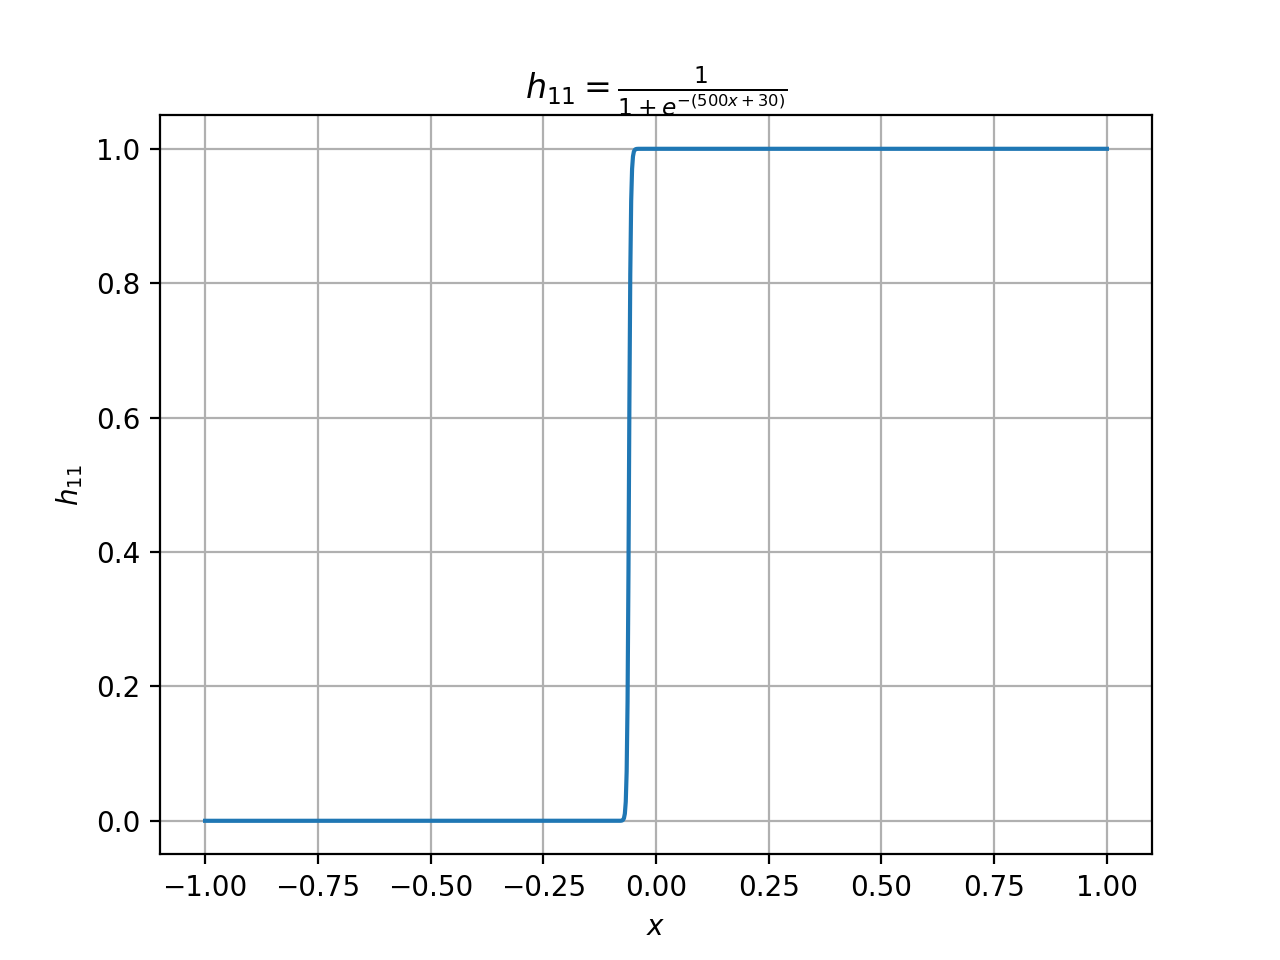
\includegraphics[scale=0.5]{q1_h11.png}
                    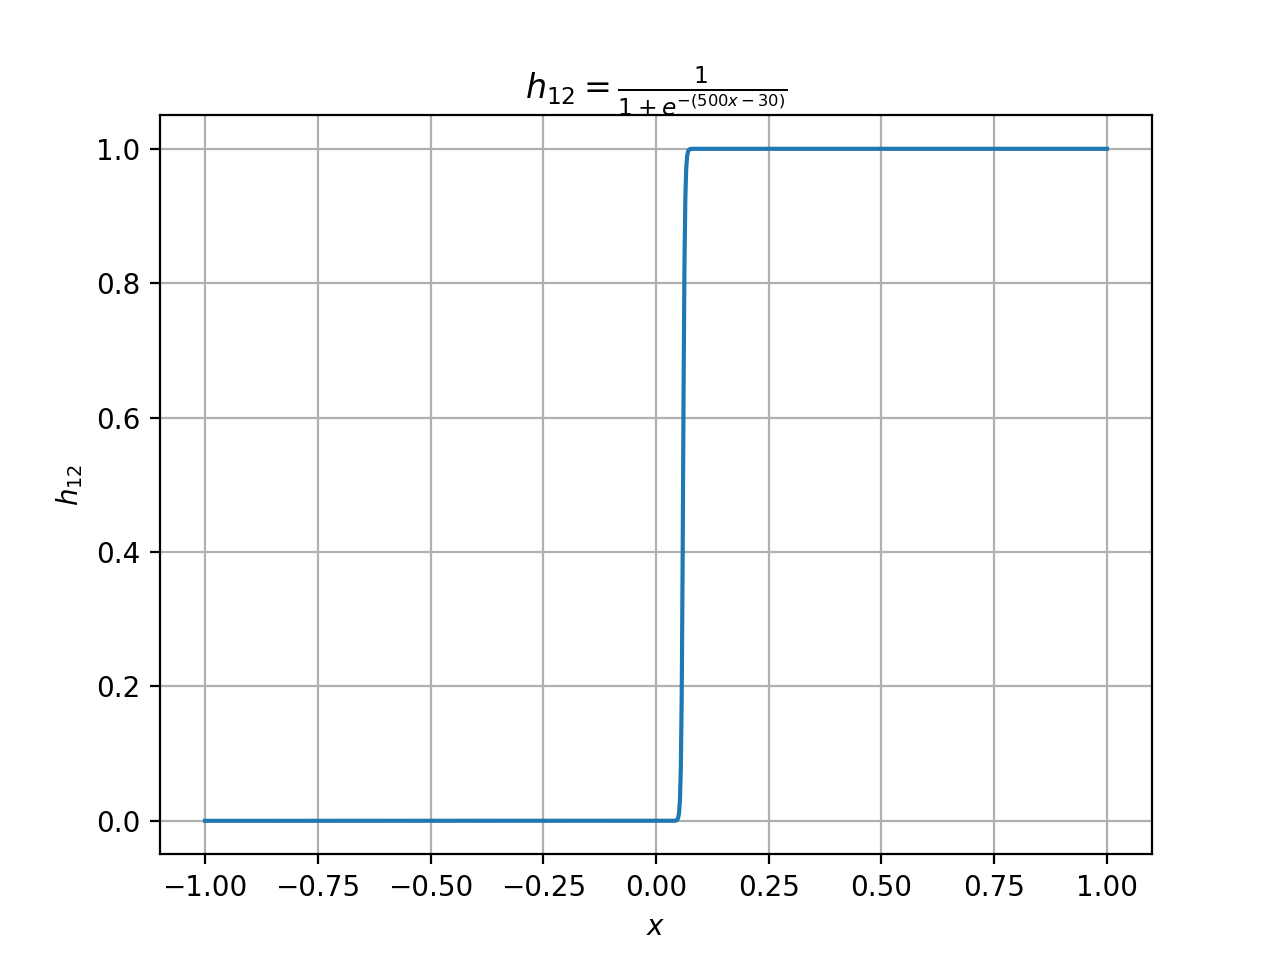
\includegraphics[scale=0.5]{q1_h12.png}
                    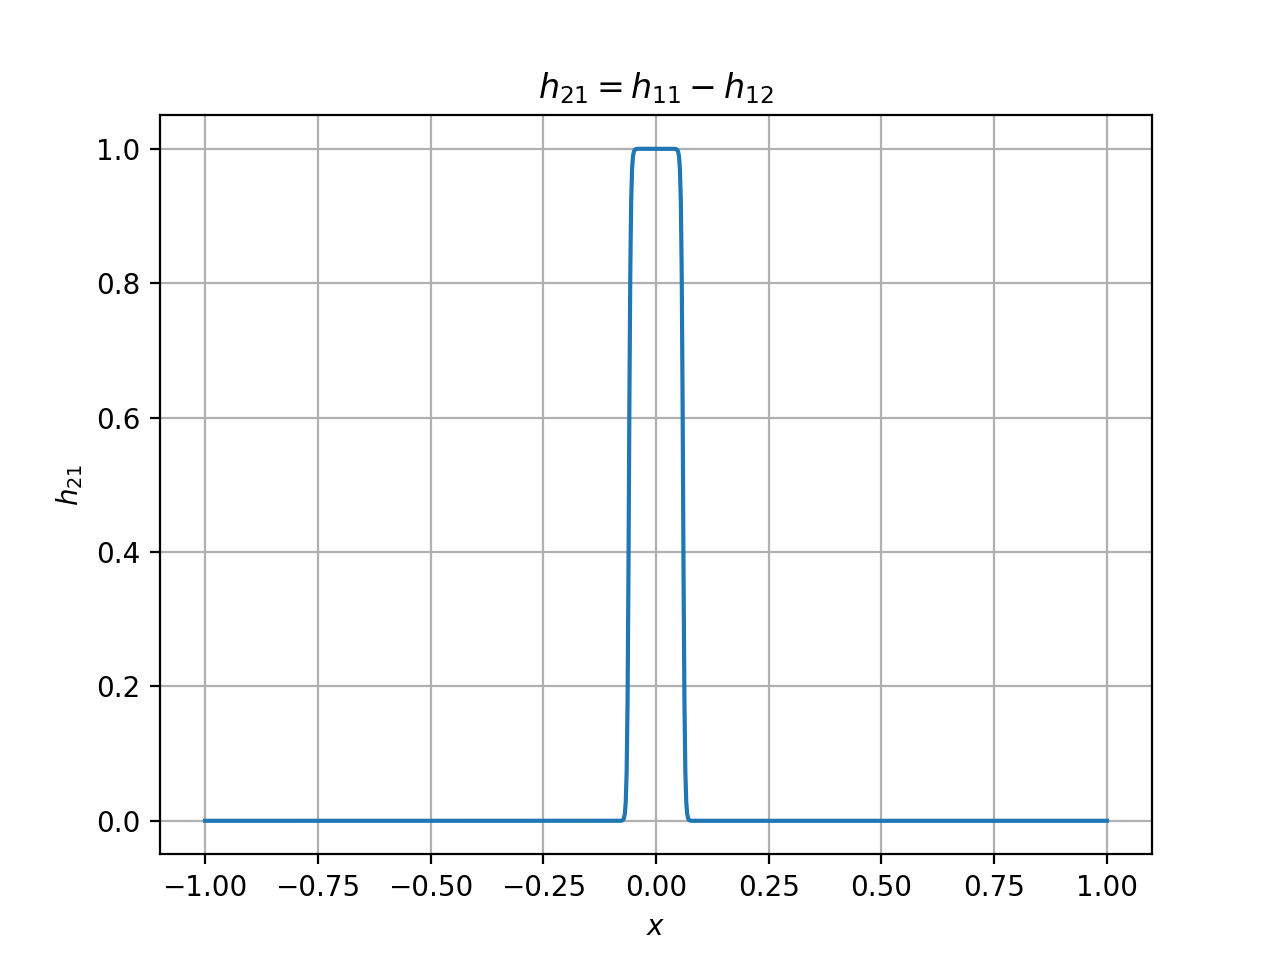
\includegraphics[scale=0.5]{q1_h21.png}
                \end{center}
            \end{solution}

            \part Now consider the variables $x_1, x_2$ and the functions $h_{11}(x_1, x_2), h_{12}(x_1, x_2), h_{13}(x_1, x_2), h_{14}(x_1, x_2)$, $h_{21}(x_1, x_2), h_{22}(x_1, x_2), h_{31}(x_1, x_2)$ and $f(x_1, x_2)$ such that   
   
                  \begin{align*}
                    h_{11}(x_1, x_2) &= \frac{1}{1 + e^{-(x_1 + 50x_2 + 100)}}  \\
                    h_{12}(x_1, x_2) &= \frac{1}{1 + e^{-(x_1 + 50x_2 - 100)}}  \\
                    h_{13}(x_1, x_2) &= \frac{1}{1 + e^{-(50x_1 + x_2 + 100)}}  \\
                    h_{14}(x_1, x_2) &= \frac{1}{1 + e^{-(50x_1 + x_2 - 100)}}  \\
                    h_{21}(x_1, x_2) &= h_{11}(x_1, x_2) - h_{12}(x_1, x_2)\\
                    h_{22}(x_1, x_2) &= h_{13}(x_1, x_2) - h_{14}(x_1, x_2)\\
                    h_{31}(x_1, x_2) &= h_{21}(x_1, x_2) + h_{22}(x_1, x_2)\\
                    f(x_1, x_2) &= \frac{1}{1 + e^{-(100h_{31}(x) - 200)}}  \\\\
                  \end{align*}
                  The above set of functions are summarized in the graph below.
                    \begin{center}
            		  \includegraphics[scale=0.35]{sig3d}
          		    \end{center} 
                  Plot the following functions: $h_{11}(x_1, x_2), h_{12}(x_1, x_2), h_{13}(x_1, x_2), h_{14}(x_1, x_2), h_{21}(x_1, x_2),$ $h_{22}(x_1, x_2), h_{31}(x_1, x_2)$ and $f(x_1, x_2)$ for $x_1 \in (-5, 5)$ and $x_2 \in (-5, 5)$
            \begin{solution}
            \begin{center}
                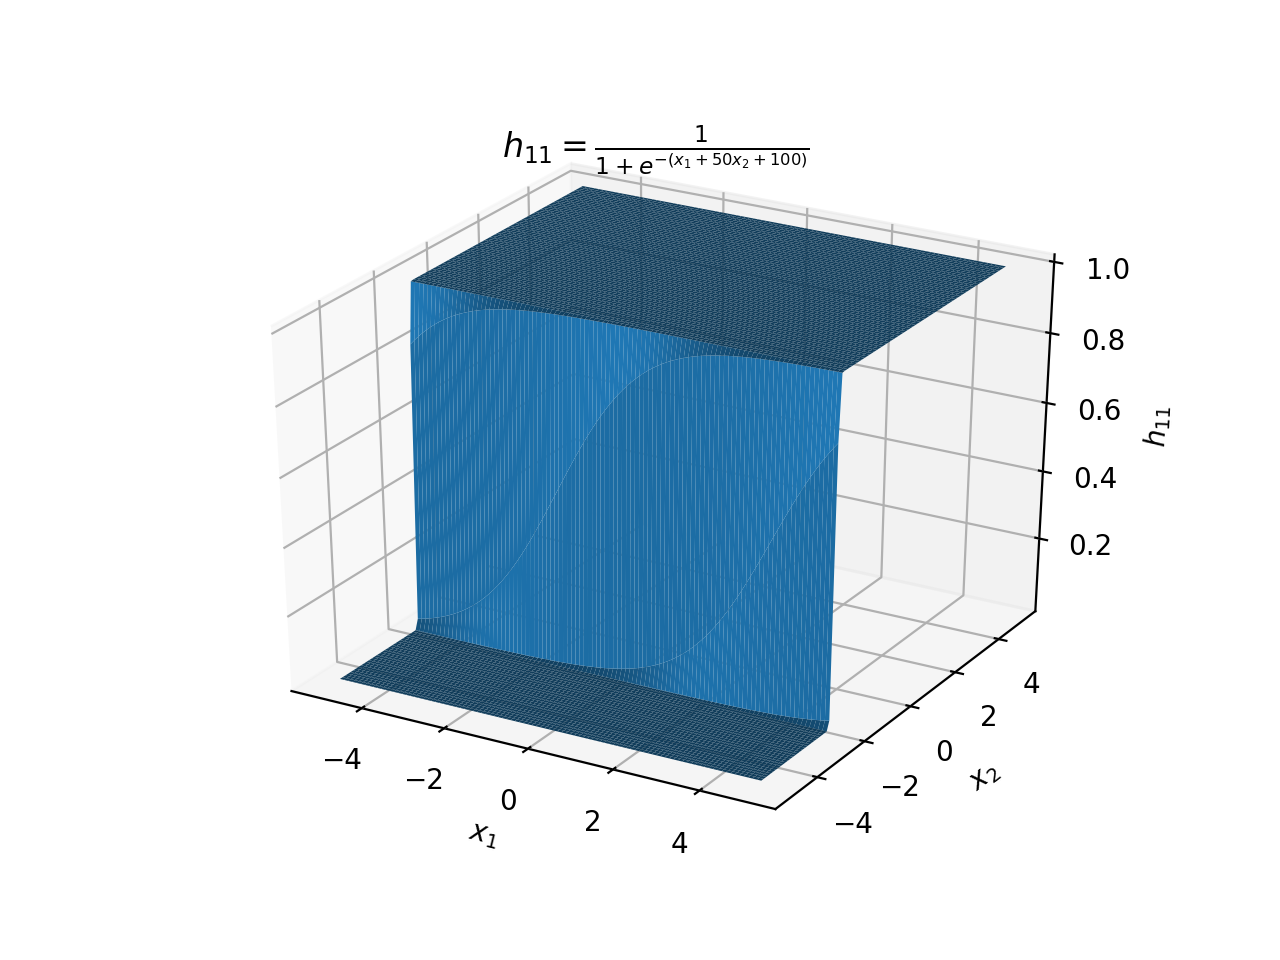
\includegraphics[scale=0.5]{q2_h11.png}
                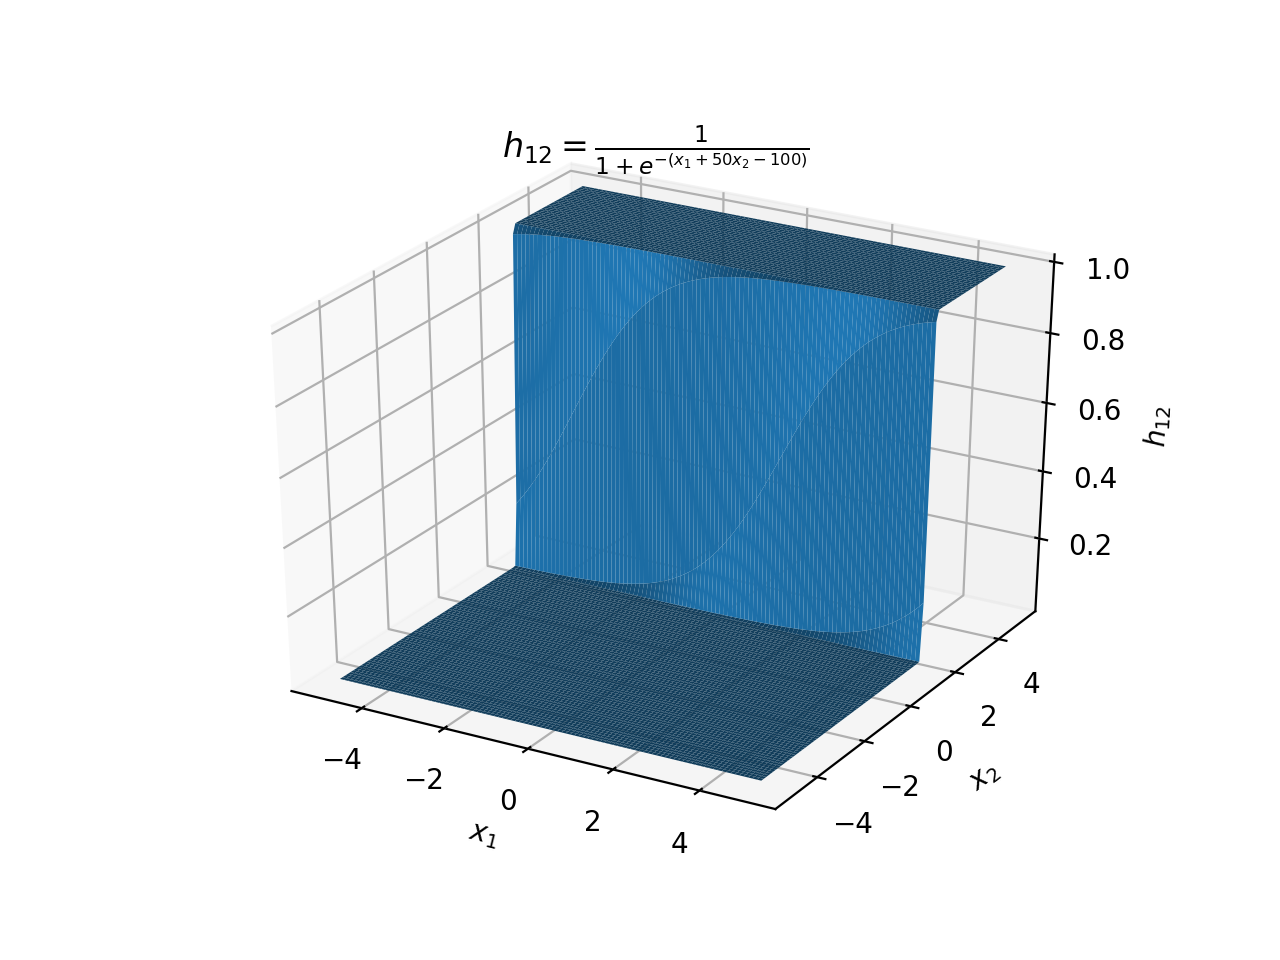
\includegraphics[scale=0.5]{q2_h12.png}
                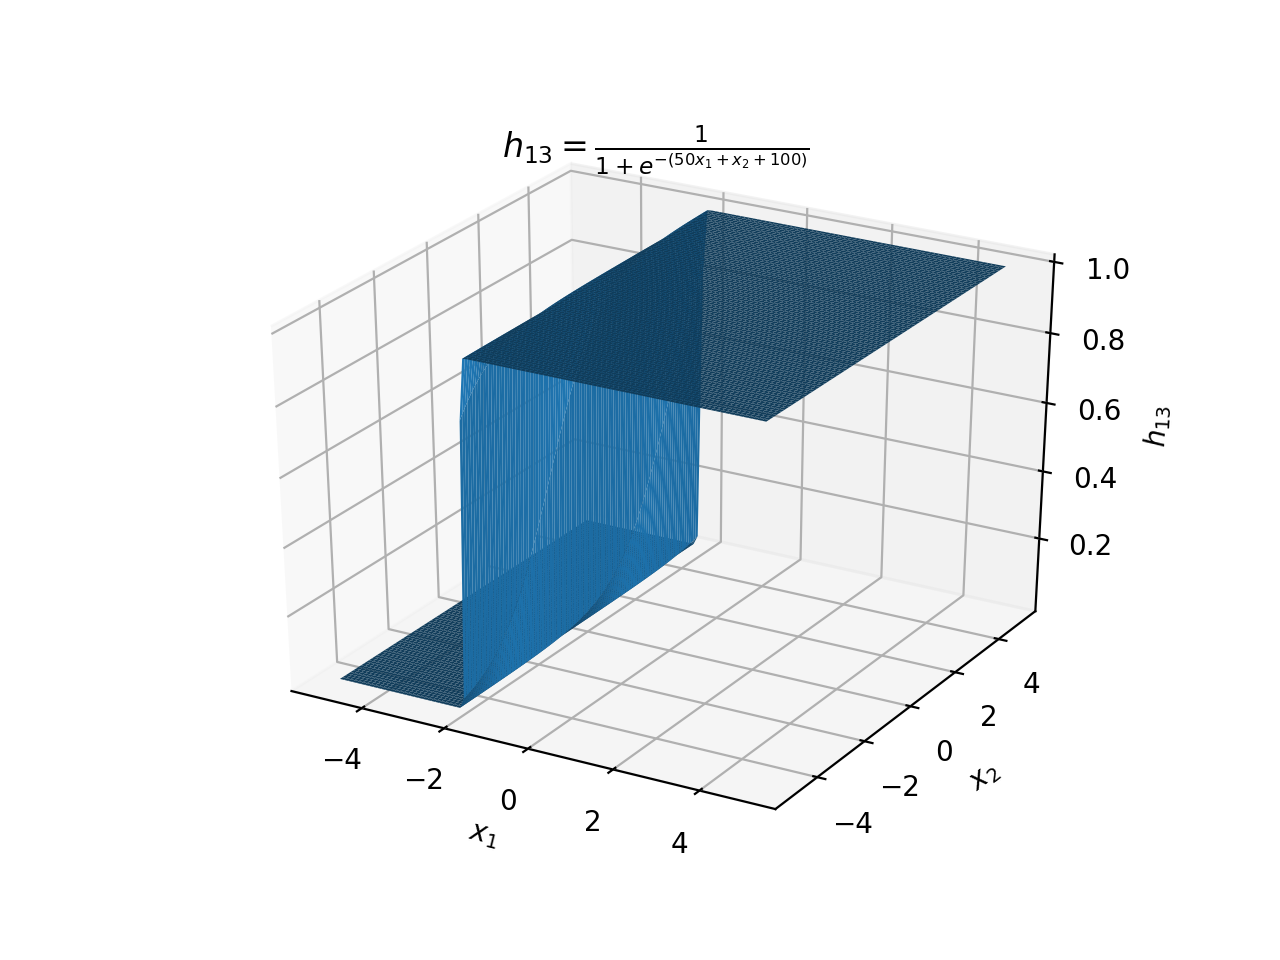
\includegraphics[scale=0.5]{q2_h13.png}
                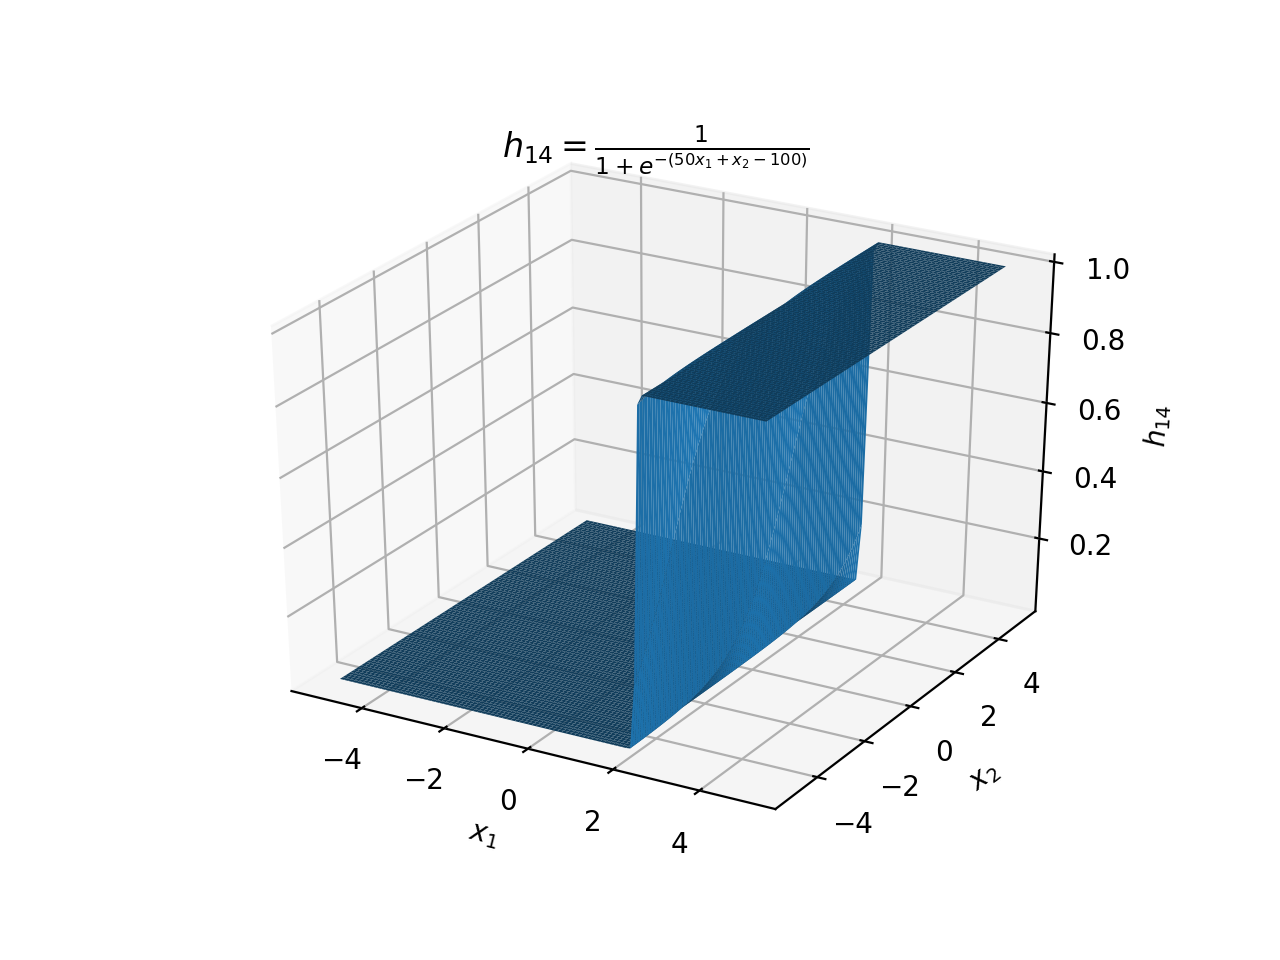
\includegraphics[scale=0.5]{q2_h14.png}
                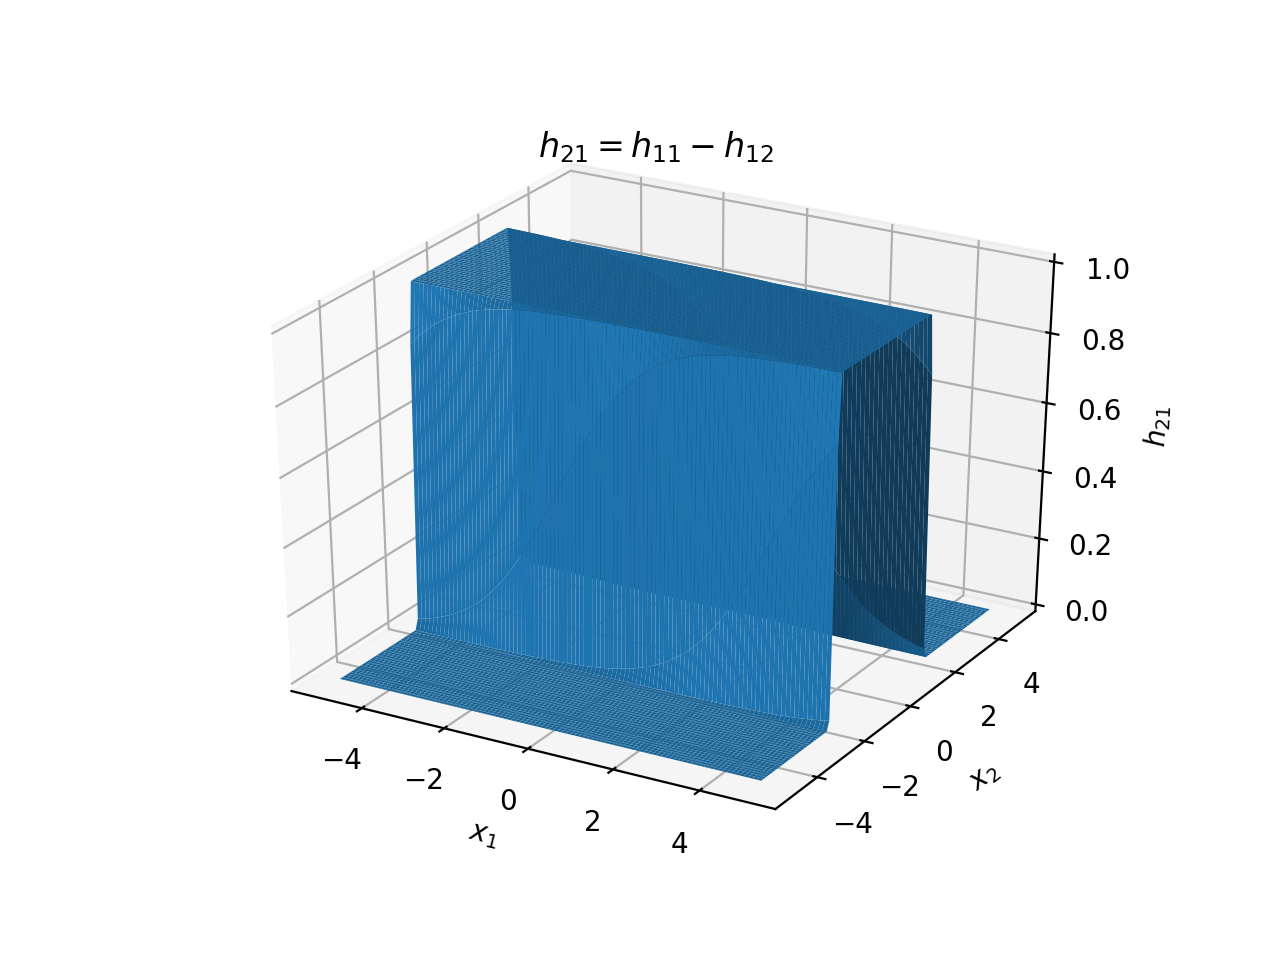
\includegraphics[scale=0.5]{q2_h21.png}
                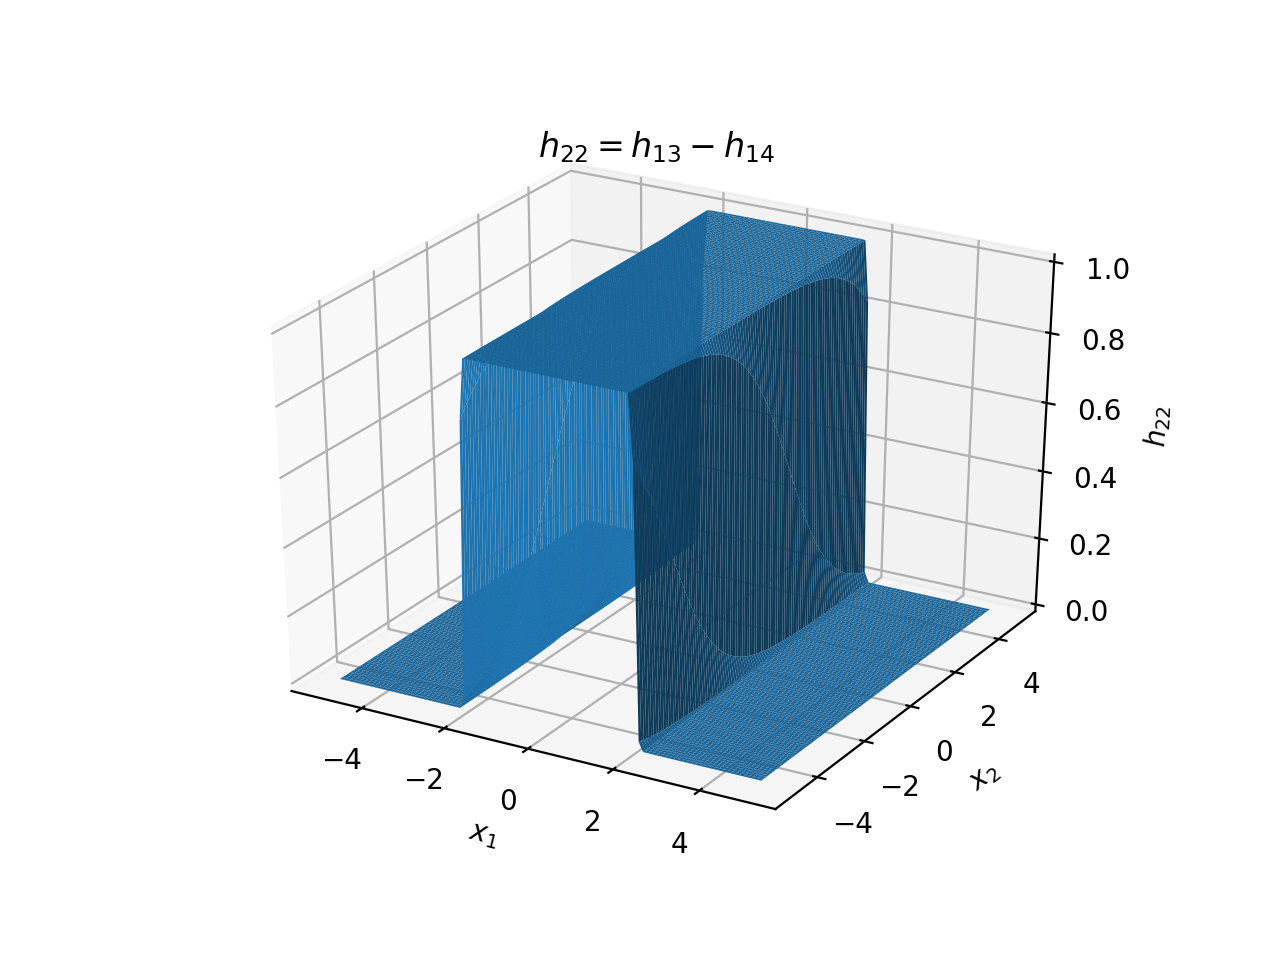
\includegraphics[scale=0.5]{q2_h22.png}
                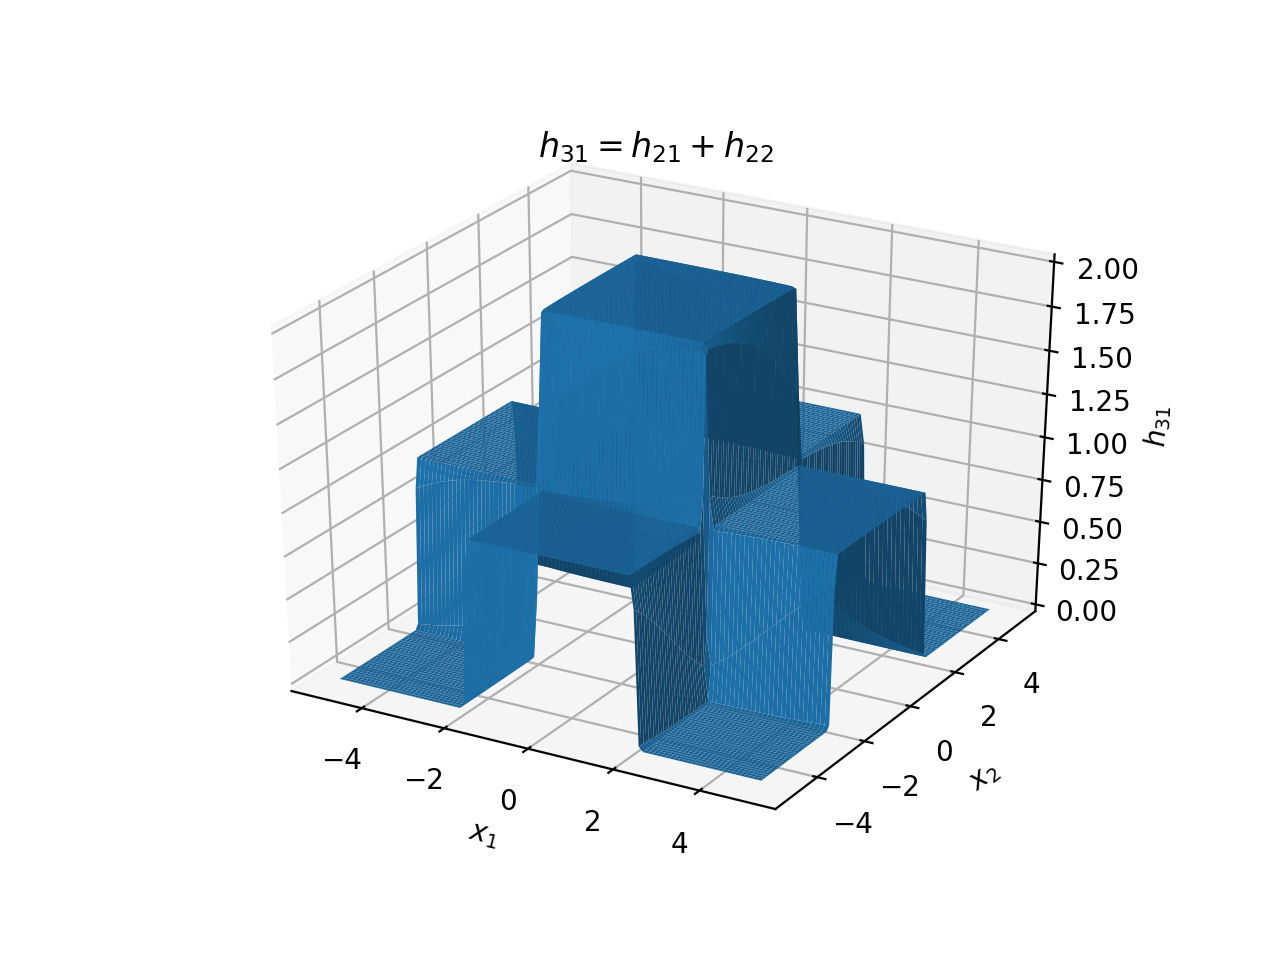
\includegraphics[scale=0.5]{q2_h31.png}
                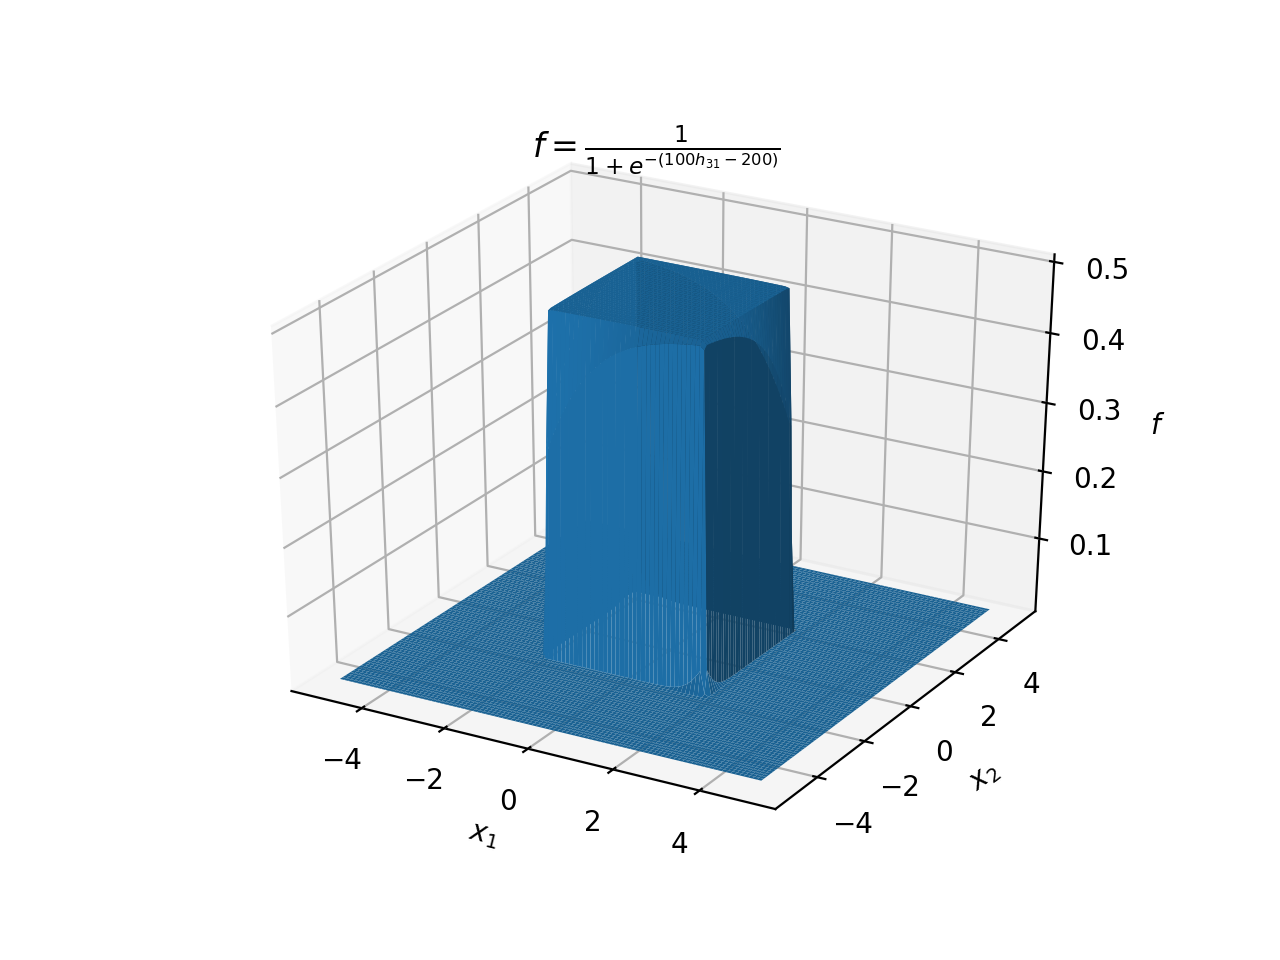
\includegraphics[scale=0.5]{q2_f.png}
            \end{center}
            \end{solution}
                 
           \end{parts}
\end{questions}             
\end{document}
